% ==============================================================================
% chapters/ch03_israel_housing_2022_2026.tex
% פרק ג': מבוא II – שוק הדיור בישראל ומבצעי הקבלן (2022–2026)
% ==============================================================================

\chapter{מבוא \en{II} – שוק הדיור בישראל ומבצעי הקבלן (\num{2022}--\num{2026})}
\label{ch:israel_housing}

בשנים \num{2022}--\num{2026} עבר שוק הדיור למגורים בישראל טלטלה מבנית חסרת תקדים בעשורים האחרונים. מעבר חד מעידן של ריבית אפסית (\pct{0.10}) לסביבת ריבית מרסנת (\pct{4.00}--\pct{4.75}), בשילוב זעזוע ביטחוני ומאקרו-כלכלי מתמשך שהאריך את משכי הבנייה, יצר דיסוננס חריף בין מחירי הדירות הנומינליים לבין כושר ההחזר החודשי של משקי הבית \cite{boi2024annual,boi2025stability}. בניגוד למחזורי האטה קודמים שבהם התאמת השוק התבצעה באמצעות ירידת מחירים נומינלית, בשנים \num{2022}--\num{2026} התבצעה ההתאמה באמצעות \textbf{הנדסה פיננסית קבלנית}: מבצעי תשלום נדחים (\num{20/80}, \num{10/90}), הלוואות בלון מסובסדות ומוטציות מימון עוקפות-רגולציה (\num{20/50/30}). פרק זה מנתח את הדינמיקה המאקרו-כלכלית שהובילה להצטברות שיא של מעל \num{85,000} דירות חדשות לא-מכורות, ממפה כמותית את פלחי השוק לפי מודל \en{TAM/SAM/SOM} מהספר \en{"}מהבעיה אל ה-\en{PDF}\en{"} \cite{segal2026prep}, ומפתח את המודל המתמטי של הנחת הערך הנוכחי הנקי (\en{NPV}) הסמויה הגלומה במבצעי הקבלנים.

\section{הזעזוע המוניטרי, קיפאון הביקושים וזינוק מלאי הדירות הלא-מכורות}
\label{sec:israel_macro_inventory}

בין שנת \num{2015} לאפריל \num{2022} פעל שוק הדיור הישראלי בסביבת ריבית בנק ישראל קרובה לאפס (\pct{0.10}--\pct{0.25}). ריבית המשכנתאות הממוצעת המשוקללת עמדה על \pct{2.1}--\pct{2.6} בלבד, מה שאיפשר למשקי בית ליטול משכנתאות בהיקף של \num{1.2}--\num{1.8} מיליון ש"ח בהחזר חודשי מתון, והזניק את מדד מחירי הדירות של הלמ"ס בכ-\pct{52} תוך שבע שנים (כולל זינוק חד של כ-\pct{20} בשנים \num{2021}--\num{2022} לבדן) \cite{boi2024annual,cbs2026dwellings}.

במקביל לזינוק במחירי הדירות, יזמי הנדל"ן ניצלו את הריבית הנמוכה לרכישת קרקעות במכרזי רשות מקרקעי ישראל (רמ"י) ובפרויקטים של התחדשות עירונית במינוף גבוה, תוך נטילת אשראי קרקע בריבית משתנה מבוססת פריים (\en{Prime + 1.5\%--3.0\%}).

המפנה המוניטרי שהחל באפריל \num{2022} שינה את כללי המשחק מן היסוד:
\begin{enumerate}[label=\textbf{\arabic*.},rightmargin=0.6cm]
  \item \textbf{זינוק עלות המימון למשקי הבית:} העלאת ריבית בנק ישראל מ-\pct{0.10} ל-\pct{4.75} בתוך \num{14} חודשים (והתייצבותה ברמת \pct{4.00}--\pct{4.50} בשנים \num{2024}--\num{2026}) הקפיצה את הריבית האפקטיבית על משכנתאות חדשות מרמה של כ-\pct{2.4} לרמה של \pct{5.4}--\pct{6.1}. עבור משכנתא ממוצעת של \num{1.5} מיליון ש"ח ל-\num{25} שנה, המשמעות הייתה התייקרות מיידית של כ-\nis{2,650} בהחזר החודשי — שחסמה אוטומטית עשרות אלפי רוכשים פוטנציאליים בשל מגבלת יחס ההחזר להכנסה (\en{PTI}) של בנק ישראל \cite{boi2025stability}.
  \item \textbf{מלחמת הסכינים התזרימית של היזמים:} ריבית הפריים בישראל זינקה מ-\pct{1.60} ל-\pct{6.25} (ובהמשך \pct{5.50}--\pct{6.00}). חברות יזמיות שנטלו הלוואות גישור למימון קרקעות ספגו הכפלה ושילוש של הוצאות המימון השוטפות. במקביל, מלחמת \en{"}חרבות ברזל\en{"} שפרצה באוקטובר \num{2023} גרמה למחסור חריף בעובדי בניין והאריכה את משך הביצוע הממוצע של פרויקט מגורים בישראל מ-\num{30} חודשים לכ-\num{38}--\num{42} חודשים \cite{boi2024annual,cbs2026dwellings}.
\end{enumerate}

\begin{figure}[htbp]
\centering
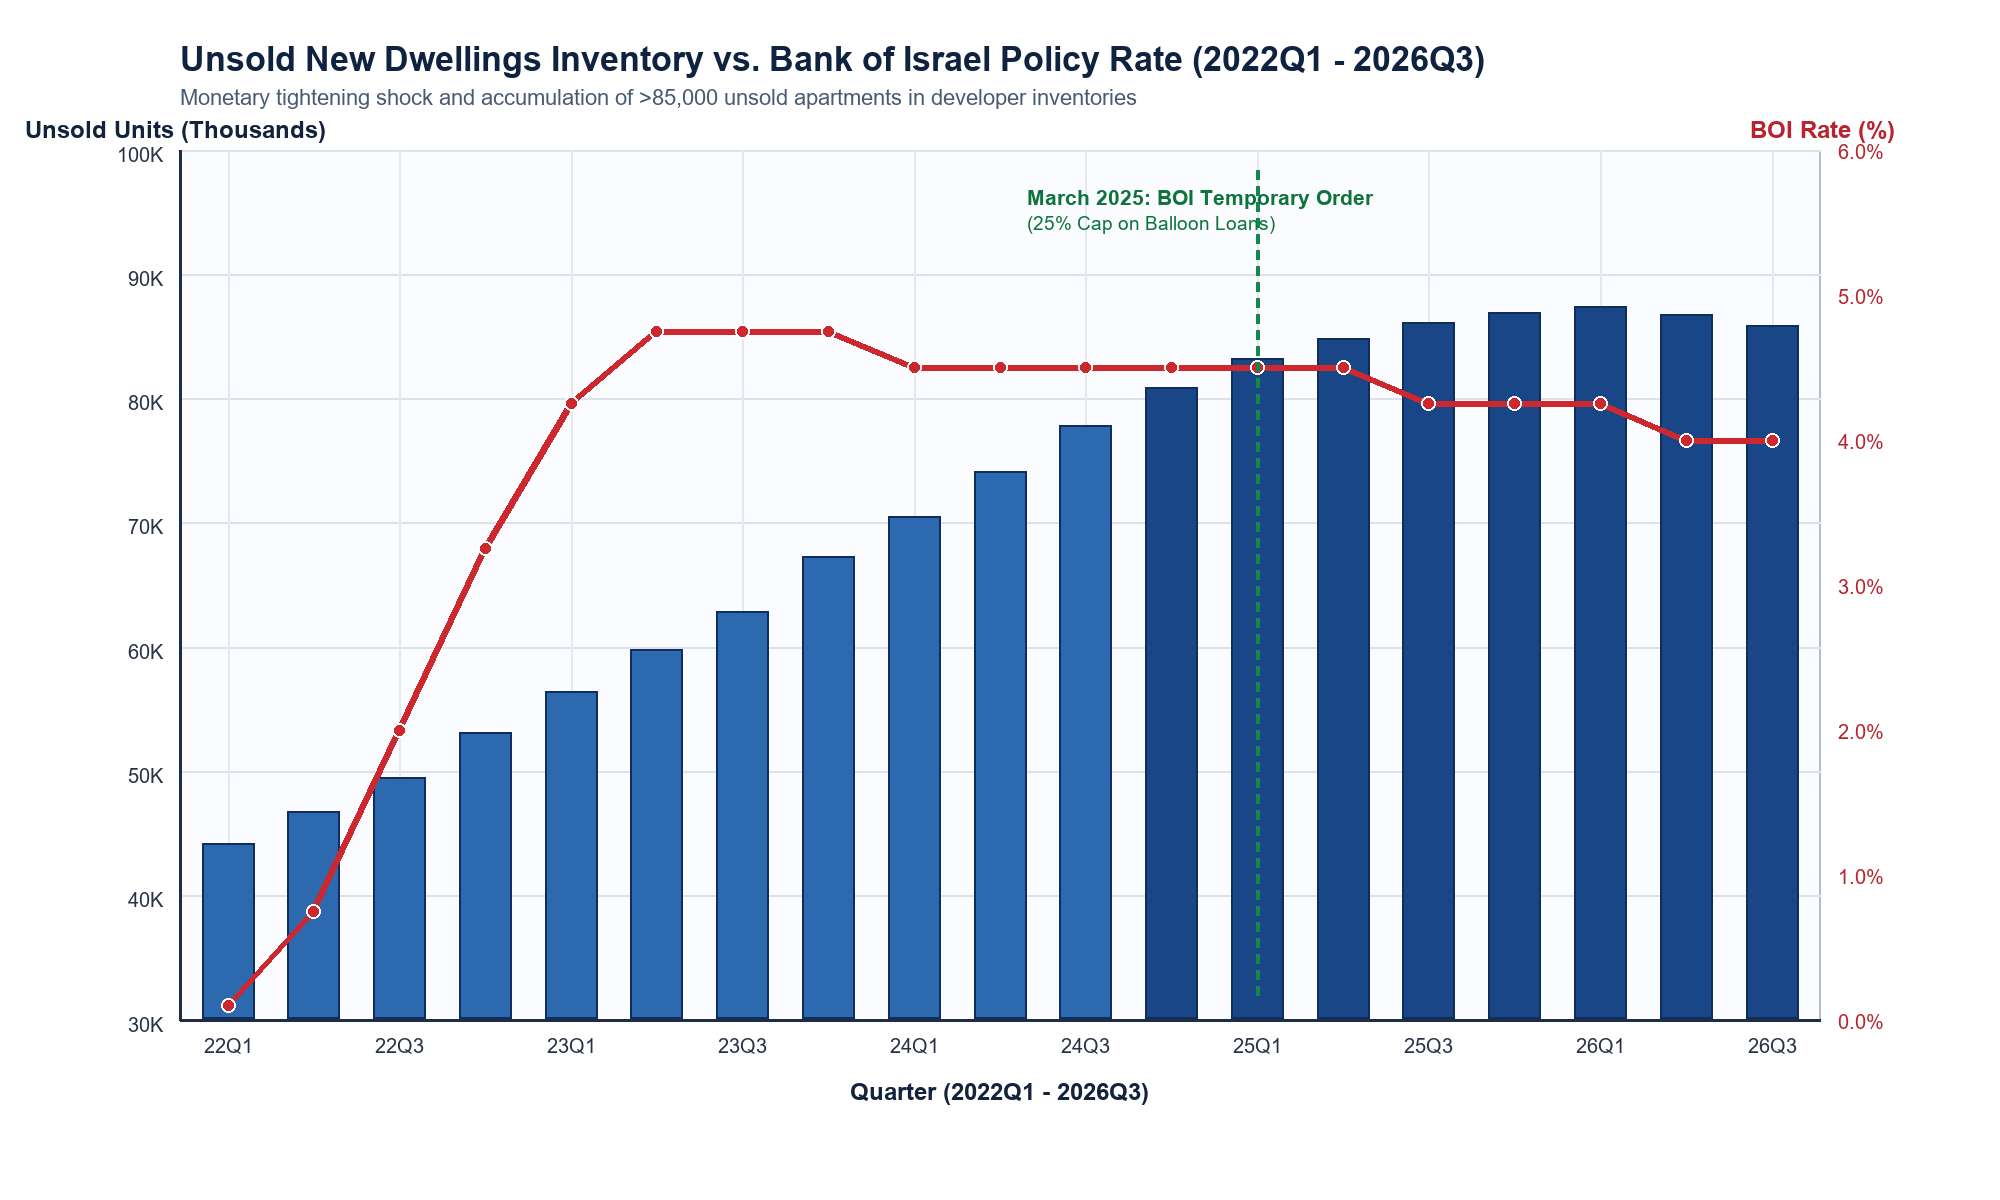
\includegraphics[width=0.96\textwidth]{fig03_israel_inventory_vs_rates.png}
\caption{התפתחות מלאי הדירות החדשות הלא-מכורות בישראל (באלפי יח"ד, ציר שמאל) מול נתיב ריבית בנק ישראל (באחוזים, ציר ימין) בשנים \num{2022}--\num{2026}: זינוק המלאי מ-\num{44,200} יח"ד לשיא של \num{87,400} יח"ד והתייצבות מעל \num{85,000} יח"ד \cite{cbs2026dwellings,boi2025stability}}
\label{fig:israel_inventory_rates}
\end{figure}

איור~\ref{fig:israel_inventory_rates} מציג את התוצאה המאקרו-כלכלית של כוחות אלו. בעוד שקצב מכירת הדירות החדשות צנח ב-\num{2023} בכ-\pct{42} לעומת שיא \num{2021}, התחלות הבנייה של פרויקטים שתוכננו ומומנו בשנות הגאות המשיכו להיכנס לצנרת הביצוע. כתוצאה מכך, מלאי הדירות החדשות הלא-מכורות שבידי הקבלנים זינק מ-\num{44,200} דירות ברבעון הראשון של \num{2022} ל-\num{67,900} דירות בסוף \num{2023}, חצה לראשונה את רף ה-\num{80,000} בסוף \num{2024}, והגיע לשיא היסטורי של \textbf{\num{87,400} דירות לא-מכורות} ברבעון הראשון של \num{2026} (ו-\num{85,900} יח"ד ברבעון השלישי של \num{2026} — שווה-ערך לכ-\num{28.5} חודשי היצע בקצב המכירות השוטף) \cite{cbs2026dwellings}.

\section{פילוח שוק תלת-שכבתי (\en{TAM / SAM / SOM}) של חשיפת מבצעי הקבלן}
\label{sec:tam_sam_som}

בהתאם להנחיות פרק \num{6.1} בספר \en{"}מהבעיה אל ה-\en{PDF}\en{"} \cite{segal2026prep}, אפיון מדויק של היקף התופעה הכלכלית מחייב פילוח כמותי תלת-שכבתי: השוק הכולל (\en{TAM -- Total Addressable Market}), השוק הנגיש (\en{SAM -- Serviceable Available Market}) ופלח השוק בר-המימוש העומד במוקד הסיכון של המחקר (\en{SOM -- Serviceable Obtainable Market}). איור~\ref{fig:tam_sam_som} וטבלה~\ref{tab:tam_sam_som} מציגים את הכימות המדויק של שלוש השכבות בשוק הדיור והאשראי הישראלי בשנים \num{2022}--\num{2026}.

\begin{figure}[htbp]
\centering
\begin{english}
\begin{tikzpicture}[font=\small]
    % Outer TAM Box
    \draw[fill=BrandLightBlue, draw=BrandNavy, line width=1.3pt, rounded corners=8pt] (0,0) rectangle (14.4,5.6);
    \node[anchor=north west, font=\normalsize\bfseries, color=BrandNavy] at (0.35, 5.3) {TAM -- Total Addressable Market (\texthebrew{כלל שוק עסקאות הדיור בישראל 2022--2026})};
    \node[anchor=north west, font=\small, color=BrandNavy] at (0.35, 4.75) {\texthebrew{היקף מצרפי: \num{385,000} עסקאות דיור (חדשות + יד שנייה) בשווי כולל של כ-\nis{885} מיליארד (\usd{242B})}};

    % Middle SAM Box
    \draw[fill=BrandLightTeal, draw=BrandTeal, line width=1.3pt, rounded corners=7pt] (0.6,0.35) rectangle (13.8,4.15);
    \node[anchor=north west, font=\normalsize\bfseries, color=BrandTeal] at (0.95, 3.85) {SAM -- Serviceable Available Market (\texthebrew{שוק הדירות החדשות מקבלן ומלאי לא-מכור})};
    \node[anchor=north west, font=\small, color=BrandTeal] at (0.95, 3.30) {\texthebrew{\num{148,000} דירות חדשות שנמכרו + \num{85,900} דירות לא-מכורות בביצוע; שווי מצרפי כ-\nis{584} מיליארד (\usd{160B})}};

    % Inner SOM Box
    \draw[fill=BrandLightRed, draw=BrandRed, line width=1.5pt, rounded corners=6pt] (1.2,0.70) rectangle (13.2,2.65);
    \node[anchor=north west, font=\normalsize\bfseries, color=BrandRed] at (1.55, 2.38) {SOM -- Target Risk Cohort (\texthebrew{פלח המטרה במחקר: עסקאות מבצעי מימון ובלון בקיר המסירות})};
    \node[anchor=north west, font=\small, color=BrandRed] at (1.55, 1.82) {\texthebrew{\textbf{\num{54,200} משקי בית} שרכשו במבצעי \num{20/80}, \num{10/90}, \num{20/50/30} והלוואות בלון (\num{2023}--\num{2026})}};
    \node[anchor=north west, font=\small\bfseries, color=BrandRed] at (1.55, 1.25) {\texthebrew{חוב נדחה לפירעון במועד המסירה (\num{2026}--\num{2027}): כ-\nis{108.4} מיליארד (\usd{29.7B}) + אשראי יזמי ממונף של כ-\nis{68} מיליארד}};
\end{tikzpicture}
\end{english}
\caption{פילוח שוק תלת-שכבתי (\en{TAM / SAM / SOM}) של שוק הדיור הישראלי ופלח הסיכון של מבצעי הקבלנים לקראת קיר המסירות (\num{2026}--\num{2027}) \cite{segal2026prep,cbs2026dwellings,boi2025stability}}
\label{fig:tam_sam_som}
\end{figure}

\begin{table}[htbp]
\caption{כימות שכבות השוק (\en{TAM / SAM / SOM}) ביחידות דיור, בשקלים חדשים ובדולרים (\num{2022}--\num{2026}) \cite{cbs2026dwellings,boi2025stability,mof2025economist}}
\label{tab:tam_sam_som}
\centering
\small
\renewcommand{\arraystretch}{1.28}
\rowcolors{2}{BrandGray}{white}
\begin{tabularx}{\textwidth}{R{1.8cm} R{3.2cm} R{2.2cm} R{2.3cm} Y}
\toprule
\rowcolor{TableHeaderBg}
\textbf{שכבה} & \textbf{הגדרת הפלח האנליטי} & \textbf{היקף ביח"ד} & \textbf{שווי מצרפי} & \textbf{משמעות מתודולוגית למחקר} \\
\midrule
\textbf{\en{TAM}} & כלל עסקאות הדיור בישראל (יד ראשונה + יד שנייה, \num{2022}--\num{2026}) & \num{385,000} יח"ד & \nis{885B} (\usd{242B}) & מסגרת המאקרו לקביעת מדדי מחירים, עומק אשראי לדיור (\nis{565B}) ויציבות בנקאית. \\
\textbf{\en{SAM}} & סקטור הבנייה החדשה (דירות שנמכרו \en{"}על הנייר\en{"} + מלאי לא-מכור של \num{85.9K}) & \num{233,900} יח"ד & \nis{584B} (\usd{160B}) & זירת הפעילות של חברות הבנייה וחשיפת האשראי הבנקאי והחוץ-בנקאי לביצוע ולקרקע. \\
\textbf{\en{SOM}} & עסקאות מבצעי מימון (\num{20/80}, \num{10/90}, \num{20/50/30}, בלון קבלן) המסתימות ב-\num{2026}--\num{2027} & \num{54,200} יח"ד & \nis{135.5B} שווי חוזי (\nis{108.4B} חוב נדחה) & \textbf{אוכלוסיית היעד של הסימולציות:} משקי הבית והיזמים שיעמדו למבחן סילוק היתרה בקיר המסירות. \\
\bottomrule
\end{tabularx}
\end{table}

\section{התפתחות מבצעי המימון: מ-\num{20/80} דרך התערבות בנק ישראל ועד מוטציות \num{20/50/30}}
\label{sec:promotions_evolution}

ניתוח כרונולוגי של שוק הראשוני בישראל בשנים \num{2022}--\num{2026} חושף אבולוציה בת שלושה שלבים במבנה חוזי המכר הקבלניים, המשקפת משחק אסטרטגי מתמשך בין היזמים לבין הפיקוח על הבנקים \cite{boi2025stability,boi2025directive,mof2025economist}:

\subsection{שלב א' (\num{2022Q4}--\num{2024Q4}): פריצת מבצעי \num{20/80}, \num{10/90} והלוואות בלון מסובסדות}
כדי להניע רוכשים לחתום על חוזים למרות זינוק הריבית, החלו הקבלנים בסוף \num{2022} להחליף את לוח התשלומים החוקי הקלאסי (שבו הרוכש משלם בשיעורים מדורגים לפי קצב התקדמות הבנייה וצמוד למדד תשומות הבנייה) בשני מנגנונים משולבים:
\begin{enumerate}[label=\textbf{\arabic*.},rightmargin=0.6cm]
  \item \textbf{דחיית תשלום ליניארית (\num{20/80}, \num{15/85}, \num{10/90} ואף \num{5/95}):} הרוכש משלם במועד החתימה \pct{10} עד \pct{20} בלבד ממחיר הדירה מההון העצמי, ופטור מכל תשלום נוסף עד לקבלת טופס \num{4} ומסירת המפתח (\num{36}--\num{42} חודשים קדימה). יתרת ה-\pct{80}--\pct{90} נדחית לתשלום אחד במועד המסירה, לרוב תוך מתן \textbf{פטור מלא או חלקי מהצמדה למדד תשומות הבנייה} על היתרה הנדחית.
  \item \textbf{הלוואת קבלן / הלוואת בלון מסובסדת (\en{Subsidized Bullet Loan}):} בפרויקטים שבהם הבנק המלווה דרש תזרים מזומנים לחשבון הליווי כבר בעת החתימה, הרוכש נטל הלוואת גישור בנקאית (\en{Bullet / Balloon}) של \pct{40}--\pct{75} משווי הדירה לתקופת הבנייה, כאשר \textbf{היזם משלם לבנק את מלוא תשלומי הריבית השוטפים} במקום הרוכש עד למועד המסירה \cite{boi2025stability,boi2025directive}. במועד המסירה פוקעת הלוואת הבלון, והרוכש נדרש לפרוע אותה באמצעות נטילת משכנתא רגילה בריבית השוק או ממכירת הדירה.
\end{enumerate}

\subsection{שלב ב' (מרץ \num{2025}): התערבות הפיקוח על הבנקים (הוראת השעה)}
לאחר ששיעור עסקאות המימון בערים מובילות חצה ברבעון הרביעי של \num{2024} את רף ה-\pct{45} מהעסקאות בדירות חדשות \cite{mof2025economist}, פרסם הפיקוח על הבנקים במרץ \num{2025} הוראת שעה מחייבת שנועדה לצנן את החשיפה המערכתית \cite{boi2025directive}. הוראת השעה קבעה שני בלמים כמותיים:
\begin{itemize}[rightmargin=0.6cm]
  \item \textbf{תוספת הקצאת הון על ליווי פרויקטים עתירי דחייה:} בפרויקטי בנייה שבהם למעלה מ-\pct{25} מחוזי המכר כוללים דחיית תשלום ליניארית (שבה שיעור התשלום במועד המסירה עולה על \pct{80} או שלוח התשלומים אינו תואם את קצב התקדמות הבנייה), חויבו הבנקים להגדיל את משקל הסיכון (\en{Risk Weight}) להקצאת הון בגין אשראי הליווי של הפרויקט.
  \item \textbf{תקרה כמותית של \pct{10} על הלוואות בלון מסובסדות:} היקף הלוואות הגישור (\en{Bullet/Balloon}) לדיור שבהן הקבלן מסבסד את הריבית הוגבל ל-\pct{10} לכל היותר מסך הביצועים החודשיים של משכנתאות חדשות בכל בנק \cite{boi2025directive}.
\end{itemize}

\subsection{שלב ג' (\num{2025Q2}--\num{2026Q4}): מוטציות עוקפות רגולציה (\num{20/50/30} ואשראי חוץ-בנקאי)}
התגובה בשוק לא הייתה הורדת מחירי המחירון של הדירות, אלא פיתוח מהיר של \textbf{מוטציות חוזיות עוקפות רגולציה} שתוכננו לעמוד פורמלית בתנאי הוראת השעה של בנק ישראל תוך שימור דחיית התשלום בפועל עבור הרוכש:
\begin{enumerate}[label=\textbf{\arabic*.},rightmargin=0.6cm]
  \item \textbf{מבנה מדורג סינתטי (\num{20/50/30} ו-\num{15/55/30}):} כדי שחוזה המכר לא יסווג כעסקה שבה \pct{80} משולמים במסירה (ובכך יפגע במכסת ה-\pct{25} של פרויקט הליווי הבנקאי), החוזה מחולק ל-\pct{20} בחתימה, \pct{50} באמצע תקופת הבנייה (למשל בחודש ה-\num{18} או ה-\num{20}), ו-\pct{30} במסירה. בפועל, עבור תשלום הביניים של ה-\pct{50}, היזם מעמיד לרוכש הלוואת גישור דרך גוף מימון חוץ-בנקאי או חברת ביטוח שותפה, או מעניק זכות דחייה חוזית מותנית עד למסירה.
  \item \textbf{הלוואות רוכשים חוץ-בנקאיות (\en{Non-Bank Buyer Bullet}):} מכיוון שמגבלת ה-\pct{10} של בנק ישראל חלה על המערכת הבנקאית בלבד, קרנות אשראי חוץ-בנקאיות וגופים מוסדיים נכנסו לוואקום והעמידו הלוואות בלון במימון של \pct{85}--\pct{90} לרוכשי דירות \en{"}על הנייר\en{"} בריביות גבוהות המסובסדות על ידי היזם מתוך תקציב השיווק של הפרויקט.
\end{enumerate}

\section{המנגנון הכלכלי והמתמטי: \en{"}מחיר מדף\en{"} נומינלי מול הנחת \en{NPV} סמויה}
\label{sec:npv_hidden_discount}

מדוע יזמי הנדל"ן בישראל מוכנים לספוג עלויות מימון וויתור על הצמדה למדד בשווי של מאות אלפי שקלים לדירה במקום להפחית ישירות את מחיר הדירה הנומינלי ב-\pct{8}--\pct{12}? התשובה טמונה במבנה המוסדי של \textbf{חשבון הליווי הבנקאי הסגור ודוח האפס}:

בליווי בנקאי סגור בישראל, הבנק מעמיד ליזם קו אשראי לביצוע הפרויקט בכפוף לשני תנאים פיננסיים קשיחים (\en{Financial Covenants}): (א) שמירה על שיעור רווח יזמי מינימלי חזוי בדוח האפס (לרוב \pct{15}--\pct{18} מהעלויות); ו-(ב) עמידה בקצב מכירות מינימלי במחיר ממוצע למ"ר שאינו נופל ממחיר הבסיס בדוח השמאי (\en{Zero Report}) \cite{boi2024annual,salelaw1974}. אם יזם מוריד רשמית את מחיר המחירון של דירה מ-\num{3.00} מיליון ש"ח ל-\num{2.70} מיליון ש"ח (\pct{-10}), שמאי הפרויקט מחויב לעדכן כלפי מטה את שווי כלל המלאי הלא-מכור בפרויקט. עדכון זה מוחק מיידית את כרית הרווח היזמי בדוח הליווי ומחייב את הבנק לדרוש מהיזם \textbf{הזרמת הון עצמי מיידית במזומן (\en{Equity Cure})} — מזומן שאין ליזמים ממונפים. לעומת זאת, כאשר היזם מוכר את הדירה במחיר חוזי נקוב (\en{Headline Price}) של \num{3.00} מיליון ש"ח במבצע \num{20/80} או בהלוואת בלון מסובסדת, המחיר הנומינלי נשמר בדוח המכירות ובדיווח לרשות המסים, בעוד שעלות הסבסוד נרשמת כ\en{"}הוצאות מימון ושיווק\en{"} הנפרסות לאורך חיי הפרויקט.

\subsection{פיתוח נוסחת הנחת הערך הנוכחי הנקי (\en{Implicit NPV Discount})}
נגדיר מתמטית את שיעור ההנחה הכלכלית הסמויה הגלומה במבצעי המימון. נסמן ב-$P_{\text{nom}}$ את מחיר החוזה הנומינלי של הדירה, וב-$T$ את תקופת הבנייה בשנים עד למסירה ($T = 3.0$ שנים, או \num{36} חודשים). בעסקת רכישה תקנית הצמודה לקצב הבנייה (\en{Benchmark Standard Contract}), הרוכש משלם סדרת תשלומים $\{\alpha_k P_{\text{nom}}\}_{k=1}^{K}$ במועדים $t_k \in [0, T]$ ($\sum_{k=1}^K \alpha_k = 1$), כאשר כל תשלום עתידי צמוד למדד תשומות הבנייה בקצב שנתי $\pi_c$, ומהוון לפי עלות ההון האלטרנטיבית / ריבית המימון השנתית $r$. הערך הנוכחי הנקי של התשלומים בעסקה תקנית (בהנחה שגם בה \pct{20} הראשונים משולמים ב-$t=0$ והיתרה נפרסת באופן שווה לאורך הבנייה) הוא:
\begin{equation}
\label{eq:pv_standard}
\text{PV}_{\text{std}} = P_{\text{nom}} \left[ \alpha_0 + \sum_{k=1}^{K} \alpha_k \left(\frac{1 + \pi_c}{1 + r}\right)^{t_k} \right]
\end{equation}

לעומת זאת, בעסקת מבצע קבלן עם דחיית תשלום ליניארית ($\alpha_0 \in \{0.10, 0.20\}$ בחתימה, ויתרה של $1 - \alpha_0$ במועד המסירה $T$ עם פטור מלא מהצמדה למדד תשומות הבנייה $\pi_c = 0$ על היתרה הנדחית), הערך הנוכחי הכלכלי שהרוכש משלם (והיזם מקבל במונחי ערך נוכחי לפני עלות מימון הבנק) הוא:
\begin{equation}
\label{eq:pv_promo}
\text{PV}_{\text{promo}}\left(\alpha_0, r, T\right) = P_{\text{nom}} \left[ \alpha_0 + \frac{1 - \alpha_0}{\left(1 + r\right)^T} \right]
\end{equation}

שיעור הנחת ה-\en{NPV} האפקטיבית הסמויה ($\delta_{\text{NPV}}$) לעומת מחיר המחירון המוצהר בעסקה צמודת-מדד מוגדר על ידי משוואה~\eqref{eq:npv_discount_rate}:
\begin{equation}
\label{eq:npv_discount_rate}
\delta_{\text{NPV}}\left(\alpha_0, r, \pi_c, T\right) = 1 - \frac{\alpha_0 + \left(1 - \alpha_0\right)\left(1 + r\right)^{-T}}{\alpha_0 + \left(1 - \alpha_0\right)\left(\frac{1 + \pi_c}{1 + r}\right)^{T/2}}
\end{equation}

\begin{figure}[htbp]
\centering
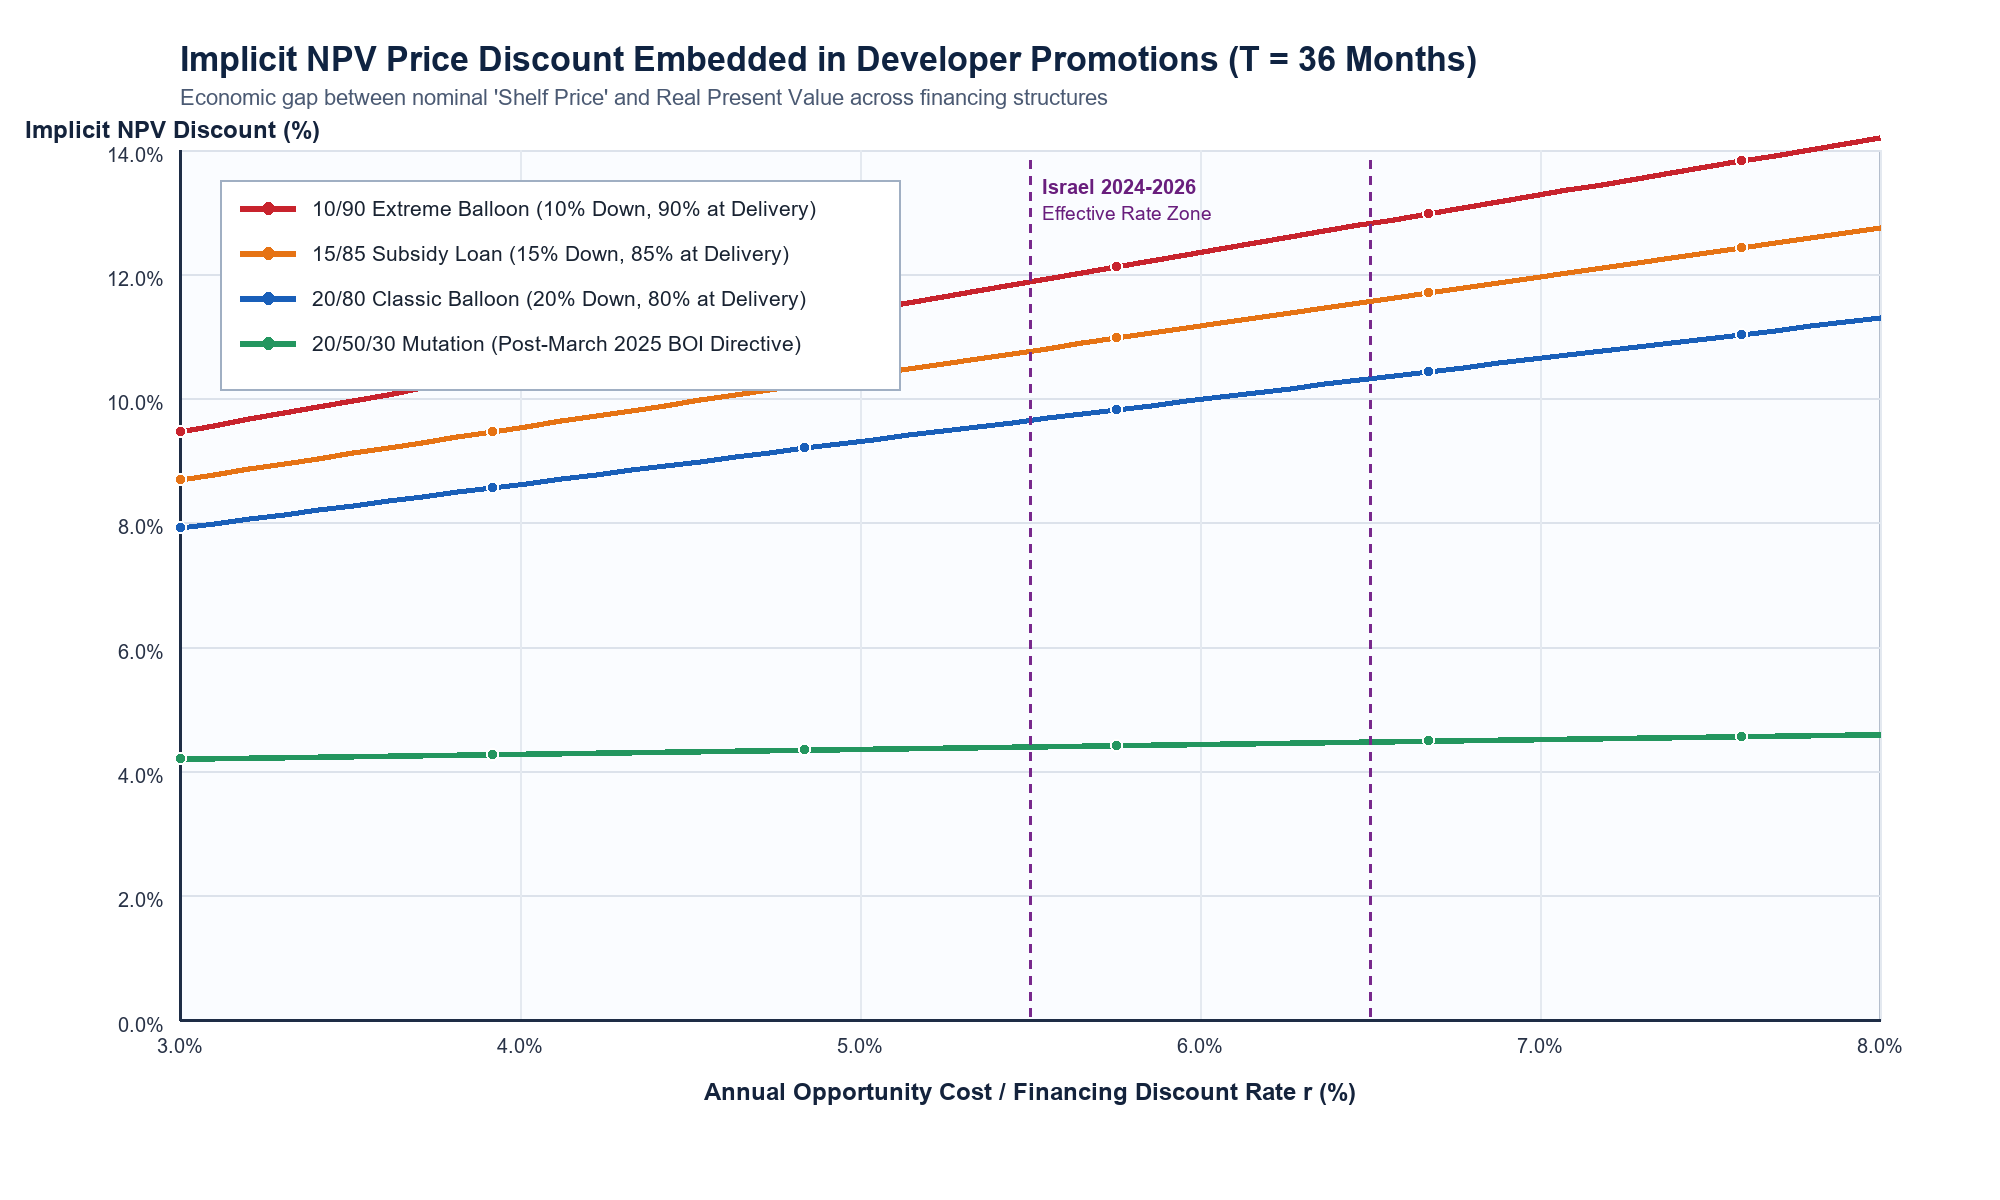
\includegraphics[width=0.95\textwidth]{fig01_npv_discount_curves.png}
\caption{עקומות שיעור ההנחה הכלכלית הסמויה (\en{Implicit NPV Discount}, $\delta_{\text{NPV}}$) כפונקציה של ריבית ההיוון השנתית ($r$) עבור שלוש ארכיטקטורות מבצעי מימון (\num{10/90}, \num{20/80} ומוטציית \num{20/50/30}) לתקופת מסירה של $T=36$ חודשים ופטור ממדד תשומות בנייה של $\pi_c=2.5\%$ לשנה}
\label{fig:npv_discount_curves}
\end{figure}

איור~\ref{fig:npv_discount_curves} וטבלה~\ref{tab:israel_promotions_anatomy} מציגים את תוצאות המודל המתמטי מתוך הרצת הסימולציה בפייתון (\en{\texttt{scripts/run\_simulations\_and\_figures.py}}). בסביבת ריבית מימון אפקטיבית של $r = 6.0\%$ לשנה ואינפלציית מדד תשומות בנייה של $\pi_c = 2.5\%$ לשנה למשך $T = 36$ חודשים:
\begin{itemize}[rightmargin=0.6cm]
  \item עסקת \textbf{\num{20/80}} מגלמת הנחת מחיר אמיתית סמויה של \textbf{\pct{9.99}} (כ-\nis{280,000} על דירה שמחירה החוזי \num{2.80} מיליון ש"ח).
  \item עסקת \textbf{\num{10/90}} (או הלוואת בלון של \pct{90} בריבית מסובסדת במלואה על ידי הקבלן) מגלמת הנחת מחיר סמויה של \textbf{\pct{12.36}} (כ-\nis{346,000} לדירה).
  \item מוטציית \textbf{\num{20/50/30}} שלאחר הוראת השעה של בנק ישראל מגלמת הנחה סמויה של \textbf{\pct{4.44}} כאשר תשלום ה-\pct{50} משולם בפועל באמצע התקופה ($t=18$ חודשים), אך שבה וחוצה את רף ה-\textbf{\pct{9.2}} כאשר תשלום הביניים ממומן באמצעות הלוואת בלון חוץ-בנקאית על חשבון היזם.
\end{itemize}

\begin{table}[htbp]
\caption{אנטומיה השוואתית של מבצעי המימון הקבלניים בישראל (\num{2022}--\num{2026}): מבנה תזרימי, הנחת \en{NPV} סמויה ומוקד סיכון ב\en{"}קיר המסירות\en{"}}
\label{tab:israel_promotions_anatomy}
\centering
\small
\renewcommand{\arraystretch}{1.28}
\rowcolors{2}{BrandGray}{white}
\begin{tabularx}{\textwidth}{R{2.5cm} R{2.8cm} R{1.9cm} R{2.1cm} Y}
\toprule
\rowcolor{TableHeaderBg}
\textbf{מבנה העסקה} & \textbf{פריסת תשלומים (חתימה / ביניים / מסירה)} & \textbf{הנחת \en{NPV} ($\mathbf{r=6\%}$)} & \textbf{חיתום בנקאי לרוכש בחתימה} & \textbf{מנגנון הכשל הפוטנציאלי בקיר המסירות (\num{2026}--\num{2027})} \\
\midrule
\textbf{חוזה תקני (ייחוס)} & \pct{20} / \pct{60} מדורג / \pct{20} (צמוד מדד תשומות) & \pct{0.00} & מלא (נטילת משכנתא מדורגת) & סיכון נמוך: יכולת ההחזר נבדקה והמשכנתא נלקחה ברובה לאורך הבנייה. \\
\textbf{ליניארי \num{20/80} (פטור ממדד)} & \pct{20} בחתימה / \pct{0} בביניים / \pct{80} במסירה & \pct{9.99} & חלקי בלבד (לרוב אישור עקרוני לא מחייב) & \textbf{הלם החזר (\en{Payment Shock}):} הרוכש נדרש לגייס \pct{80} במשכנתא אחת בריבית גבוהה בעת המסירה. \\
\textbf{קיצון \num{10/90} / \num{15/85}} & \pct{10}--\pct{15} בחתימה / \pct{0} בביניים / \pct{85}--\pct{90} במסירה & \pct{12.36} & היעדר חיתום מחייב; משקיעי \en{"}פליפ\en{"} & \textbf{מלכודת \en{LTV} ו-\en{PTI}:} משקיע או משפר דיור שמוגבל ל-\pct{50}--\pct{70} משכנתא אינו יכול להשלים את העסקה ללא מכירה. \\
\textbf{הלוואת בלון קבלן מסובסדת} & \pct{15}--\pct{20} הון עצמי + \pct{65}--\pct{80} בלון בנקאי בריבית על חשבון היזם & \pct{9.80}--\pct{11.50} & חיתום בנקאי מראש על הלוואת הגישור & \textbf{סיכון מחזור (\en{Rollover Risk}):} פקיעת הבלון במסירה מחייבת מעבר להחזר חודשי מלא של קרן וריבית. \\
\textbf{מוטציית \num{20/50/30} (אחרי מרץ \num{2025})} & \pct{20} בחתימה / \pct{50} בחודש \num{18} (בלון חוץ-בנקאי) / \pct{30} במסירה & \pct{4.44} (או \pct{9.20} בסיבסוד חוץ-בנקאי) & עוקף את מגבלת ה-\pct{25} וה-\pct{10} של בנק ישראל & \textbf{זליגת סיכון לאשראי חוץ-בנקאי:} מינוף כפול של הרוכש והיזם מול קרנות מימון פרטיות בריבית גבוהה. \\
\bottomrule
\end{tabularx}
\end{table}

\begin{warningbox}[העיוות הסטטיסטי והמימוני הכפול של מבצעי הקבלן]
הניתוח המתמטי בפרק זה חושף כי מבצעי המימון הקבלניים בשנים \num{2022}--\num{2026} ייצרו שני עיוותים מערכתיים במקביל:
\begin{enumerate}[label=\textbf{\arabic*.},rightmargin=0.5cm]
  \item \textbf{עיוות מדידת האינפלציה ומדד מחירי הדירות:} מאחר שהלמ"ס ורשות המסים קולטים את מחיר החוזה הנומינלי ($P_{\text{nom}}$) ללא ניכוי הנחת ה-\en{NPV} הסמויה ($\delta_{\text{NPV}} \approx 10\%$), מדד מחירי הדירות הרשמי בשנים \num{2023}--\num{2025} הציג יציבות או עלייה מדומה בשעה שהמחיר הכלכלי הריאלי בשוק הראשוני ירד \cite{mof2025economist,ita2025carman}.
  \item \textbf{דחיית החיתום הבנקאי האמיתי למועד האכלוס (\en{Deferred Underwriting}):} בעסקאות \num{20/80} ו-\num{10/90} ליניאריות (שאינן מבוססות על הלוואת בלון בנקאית שנחתמה מראש), הרוכש אינו נוטל משכנתא במועד החתימה. בדיקת כושר ההחזר המחייבת לפי יחס ה-\en{PTI} והערכת שמאי הבנק למשכנתאות נדחות ב-\num{36} חודשים למועד המסירה (\num{2026}--\num{2027}) — בדיוק בנקודת הזמן שבה מצטברות מעל \num{85,000} דירות לא-מכורות מתחרות.
\end{enumerate}
\end{warningbox}
